\section{Network-Wide Telemetry System}
\label{sec:mechanism}

In this section, we first describe the technical challenges of building a network-wide telemetry system with INT and then provide our own design to conquer these challenges via the \emph{separation of mechanism and policy}.

\subsection{Challenging Issues}
\label{subsec:challenge}

\textbf{Uncontrollable probing path.}
As an underlying primitive, INT merely defines how to extract device-internal states using probe packets. However, the probe packet itself cannot proactively decide which path to monitor since it does not have any path-related prior knowledge. If the INT header is embedded in an IP packet, the probing path will be passively decided by its destination IP address together with the routing table in each network device, leaving probing path totally \emph{uncontrollable} by INT agents. Given the uncontrollable probing path, it is not easy to work out purposive strategies to generate multiple probing paths for achieving network-wide telemetry. 

\textbf{Telemetry overhead.}
During traffic monitoring, we need periodically perform the INT operation at all devices and notify the controller about the underlying traffic status. However, straightforwardly conducting INT at each device or device chain incurs significant performance \emph{overhead}: (1) INT will inject probes into the network, which will occupy a fraction of link bandwidth (the finer INT sampling granularity, the more bandwidth will be consumed). (2) INT agents must be deployed for probe generation and collection (the more separated INT paths, the higher number of INT agents need be deployed). Besides, as the INT agent number grows, the controller will suffer from a performance penalty for handling increased telemetry workload sent from the INT agents.

\textbf{Synchronized multi-path monitoring.}
% 集中式控制器需要采集每条path上的链路状态信息才能进行全网状态的评估。然而如果path的长度存在较大的差异,那么集中式控制器必须等待最长path上的INT包返回之后才能开始全网状态评估,这将大大降低全网链路状态采集的时效性。为此,我们希望INT path的长度是balanced。
In each monitoring round, the centralized controller cannot evaluate the global network view until the probe packets from all the monitoring paths are collected. That is to say, if one path is much longer than the others, the controller has to delay the control decision making until the return of the last probe packet from the longest path, which does degrade the timeliness of centralized control. Hence, \emph{balanced} path generation is preferable.

\subsection{Design Space Analysis}
As an auxiliary function for better network management, a cost-effective telemetry implementation is welcome. To enable network-wide telemetry, \emph{all} edges of the network graph should be covered by the probing paths\footnote{Since the INT probe packet can only collect the queue depth or the queuing latency from the network interfaces it travels through, constructing monitoring paths into a spanning tree or a Steiner tree is insufficient for obtaining the network-wide link status at the controller side.}. To reduce unnecessary bandwidth cost, \emph{non-overlapped} probing paths are preferable. To lessen the processing overhead of the telemetry workload at the controller, the path number should be kept as \emph{small} as possible. To retain the timeliness of centralized control, the path length should be as \emph{balanced} as possible. To simultaneously satisfy the above design goals, the start/end node of each probing path need be carefully planned. However, as mentioned earlier, the original INT lacks of the ability to specify the route the probe packet takes though the network, which is the exact prerequisite for accurate path planning. Here, we propose \emph{INT-path}, a framework for network-wide telemetry, by decoupling the system into a routing \emph{mechanism} and a route generation \emph{policy}. The underlying mechanism allows network operators/INT agents to specify a particular path for monitoring, addressing the uncontrollable path issue (\S\ref{subsec:mechanism}). The policy built upon the mechanism generates multiple INT paths to traverse the entire network and a good policy is expected to minimize the telemetry overhead (\S\ref{subsec:policy} and \S\ref{sec:algorithm}).

\subsection{Source Routing-based Path Monitoring (Mechanism)}
\label{subsec:mechanism}

We address the uncontrollable path issue via the technique of \emph{source routing} (SR)~\cite{sunshine1977source}. Fig.~\ref{fig:demand_int1} shows the source routing-based telemetry architecture as well as the probe packet header format. In computer networking, source routing allows a sender of a packet to specify the route the packet takes though the network, usually by labeling the route onto the packet header. In contrast, in non-source routing protocols, packets are forwarded by routers based on the destination addresses. Although source routing is not a new technique, we are the \emph{first} to couple it with the INT probe using the P4 language~\cite{bosshart2014p4} to implement user-specified/on-demand path monitoring.




\begin{figure}
\centering
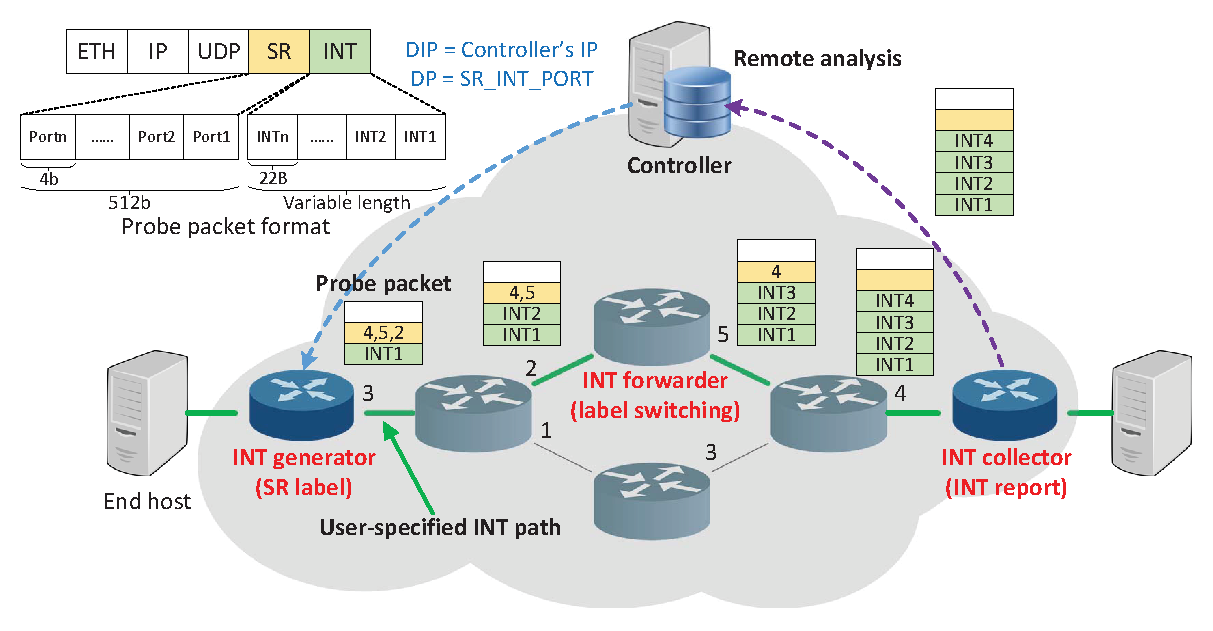
\epsfig{file=figure/demand_int1.eps, scale=0.435}
\vspace{-0.3cm}
\caption{Source routing-based path monitoring.}
\label{fig:demand_int1}
\vspace{-0.3cm}
\end{figure}

\textbf{Packet header format.}
In Fig.~\ref{fig:demand_int1}, we use a UDP packet to carry the SR-INT payload. To inform the packet parser that it is an SR-INT probe, the destination port (DP) number is set to ``SR\_INT\_PORT''. Above the UDP header, we reserve 512-bit for the SR label stack. We allocate 4-bit for each SR label to denote the router output port ID thus can maximally support 16 output ports for each router. Above the \emph{fixed-length} SR label stack, we allocate a \emph{variable-length} INT label stack. Each INT label occupies 22B containing the information such as device ID, ingress/egress port, egress queue depth. Since P4 currently does not well support parsing double variable-length stacks in the packet header, we statically allocate the SR label stack and use the right shift operation (``$\gg$'') to perform the ``stack pop'' behavior. The destination IP (DIP) address of the probe packet is set using controller's IP to guarantee that the probe packet will finally be forwarded to the controller for further analysis. Notice that although we design a customized header format for the probe packets, the network devices can still correctly forward these packets given \emph{protocol-independent forwarding}~\cite{bosshart2014p4} is supported.

\textbf{Forwarding behaviors.}
In the SR-based telemetry architecture, we propose three types of logic routers with different functionalities: the \emph{INT generator}, the \emph{INT forwarder} and the \emph{INT collector}. A physical device can simultaneously act as an INT generator and an INT collector. In other words, a physical device can be at the end of one monitoring path while at the start of another monitoring path at the same time.

The \emph{INT generator} is responsible for spawning the SR-INT probe packets at the first hop of the monitoring path. Since packet generation directly from the data plane is currently undefined by the P4 language, we consider a workaround to periodically generate ``empty'' probes from the outside by either the router/switch CPU or a server attached to the network device. When the probe arrives at the data plane, the INT generator will rewrite its packet header to add the SR label stack and its local INT information using \texttt{header.setValid()} and then forward the packet. Specifically, the INT generator will push the output port IDs into the SR label stack in the packet header. The sequence of the output port IDs (\ie, how to forward the packet across the network) is predetermined at the controller via centralized route calculation. 

The \emph{INT forwarder} performs packet forwarding of either the SR-INT probes or the ordinary traffic, according to the DP number of the incoming traffic. If the DP is ``SR\_INT\_PORT'', the INT forwarder will perform label switching (similar with MPLS) and forward the packet only according to the output port ID popped from the SR label stack (the DIP is no longer used in this case). The SR label is popped once at a router by right shifting the SR header by 4 bits at each hop. Besides, the INT forwarder will also push its local INT information into the INT label stack before forwarding the probe. 

At the last hop of the monitoring path, since the DIP is filled with controller's IP address, the \emph{INT collector} will finally forward the probe packet to the controller for further analysis.

\subsection{INT Path Planning for Graph Coverage (Policy)}
\label{subsec:policy}

Based on the SR-based telemetry mechanism, we can accurately control each probing path thus can develop diverse INT path planning algorithms for \emph{non-overlapped} INT path generation that covers the \emph{entire} network graph. Here, we first propose a simple algorithm based on \emph{depth-first search} (DFS), followed by a more sophisticated one based on \emph{Euler trail} which generates the \emph{optimal} result.

When traversing a tree or a graph, DFS starts at the root and explores as far as possible along each branch before backtracking. The basic idea of the DFS-based path planning algorithm is to consecutively add the visited vertices into the current path before backtracking; if we have nowhere to go and have to backtrack, we just create a new path and add the \emph{fork} vertex (the first vertex along the backtracking path that has unvisited edges) as the first node in the new path. After all the vertices are visited in the DFS order, we can extract multiple non-overlapped paths covering the entire graph.



Fig.~\ref{fig:dfs} shows a \emph{recursive} version of the DFS-based path planning algorithm. For each visited vertex, we will choose one of its unvisited edges for depth-first traversal (line 6-7 in Fig.~\ref{fig:dfs}). If we have chosen an unvisited edge, we will mark it as visited (line 8-9). We will explore as far as possible and add the visited vertices into the current INT path before backtracking occurs (line 17). On backtracking, we will create a new path from the fork vertex as the current path (line 12). In Fig.~\ref{fig:dfs}, we use the technique of recursion (line 19) to perform backtracking and leverage an additional \emph{flag} to locate the fork vertex during recursion. When a backtracking occurs during DFS, the current function call will return with \emph{true} (line 22) as its return value (which will be assigned to the bool variable \emph{flag} in its caller function in line 19). When the \emph{flag} is \emph{true} (line 10) and there is at least one unvisited edge (line 7), the currently visited vertex can be identified as a fork vertex (line 12-13) according to the previous definition. The recursion will finally halt when all the edges are visited. Besides, the first vertex $v_0$ of the depth-first traversal should be specially treated as a boundary case (line 1-3) and we have to invoke PathPlan($v_0$, \emph{true}) to start the algorithm. The run-time complexity of the algorithm is $O(V^2)$, similar with the classic DFS, if the graph is implemented with an adjacency matrix.

\begin{figure}
\centering
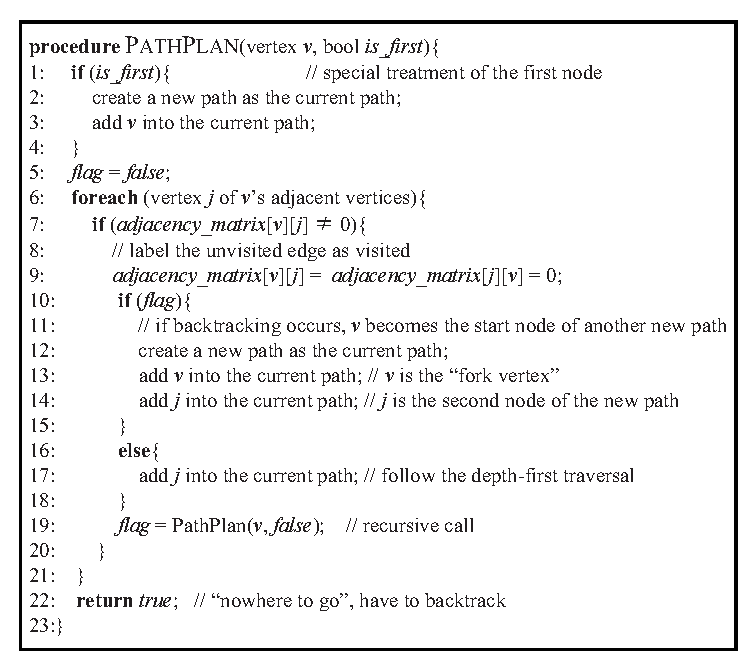
\epsfig{file=figure/algorithm.eps, scale=0.71}
\vspace{-0.2cm}
\caption{DFS-based INT path planning algorithm (a recursive version).}
\label{fig:dfs}
\vspace{-0.2cm}
\end{figure}

Fig.~\ref{fig:graph} shows an algorithm example on a network graph of five devices. After PathPlan($v_0$, \emph{true}) is invoked, $v_0$ is pushed into the call stack, path1 = \{$v_0$, $v_1$\} and the edge between $v_0$ and $v_1$ is marked as visited. The path1 expands as more and more vertices are visited in the DFS order. When path1 expands to \{$v_0$, $v_1$, $v_2$, $v_3$, $v_1$\}, we have nowhere to go and have to backtrack. At this time, we pop $v_1$ from the stack and return to $v_3$, which has an unvisited edge to $v_4$ (notice that the call stack push/pop operations are implicitly performed during recursion). Then, we identify $v_3$ as the \emph{fork} vertex because it is the first vertex along the backtracking path that has unvisited edges. Based on $v_3$, we create a new path as path2 = \{$v_3$, $v_4$\}. When path2 expands to \{$v_3$, $v_4$, $v_2$\}, we have again nowhere to go and have to backtrack. But at this time, although we check all the vertices popped from the call stack, we still cannot find any fork vertex. The recursion halts when the call stack finally becomes empty. At last, we extract two non-overlapped INT paths (\ie, path1 and path2).


\begin{figure*}[t]
    \centering
    \begin{minipage}[b]{0.345\textwidth}
        \centering
        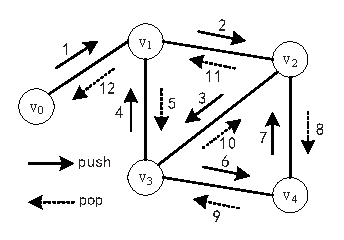
\includegraphics[width=0.75\textwidth]{figure/graph.eps} 
        \vspace{-0.2cm}
        \caption{Depth-first graph traversal.}\label{fig:graph}
    \end{minipage}
    % \hfill
    \hspace{0.0in}
    \begin{minipage}[b]{0.64\textwidth}
        \centering
        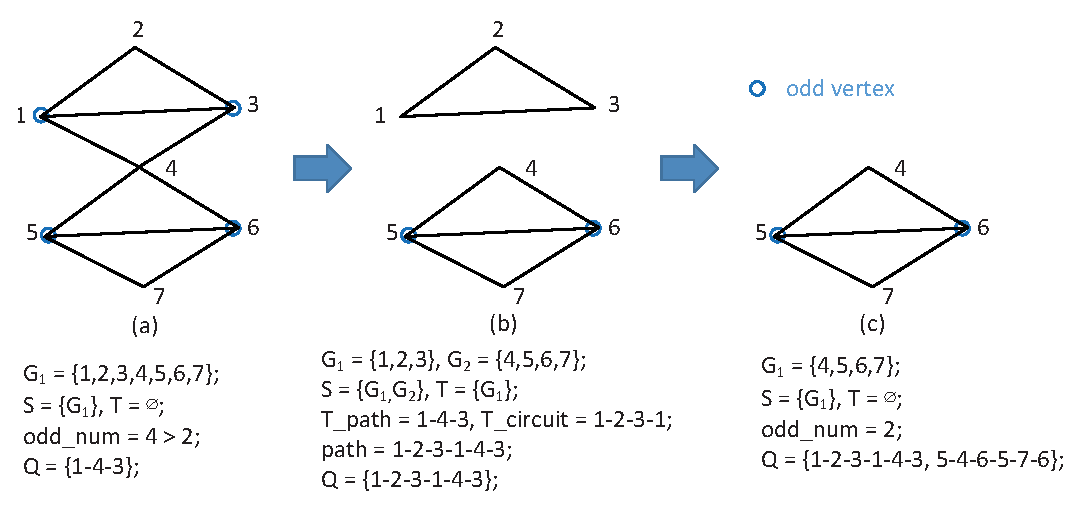
\includegraphics[width=0.78\textwidth]{figure/euler.eps}
        \vspace{-0.2cm}
        \caption{Path extraction process of the Euler trail-based algorithm.}\label{fig:euler}
    \end{minipage}
    \vspace{-0.45cm}
\end{figure*}









